
%%%%%%%%%%%%%%%%%%%%%%%%%%%%%%%%%%%%%%%%%%%%%%%%%%%%%%%%%%%%%%%%%%%%%%%%%%%%%%
% Copyright (c) 2003-2013 by University of Queensland
% http://www.uq.edu.au
%
% Primary Business: Queensland, Australia
% Licensed under the Open Software License version 3.0
% http://www.opensource.org/licenses/osl-3.0.php
%
% Development until 2012 by Earth Systems Science Computational Center (ESSCC)
% Development since 2012 by School of Earth Sciences
%
%%%%%%%%%%%%%%%%%%%%%%%%%%%%%%%%%%%%%%%%%%%%%%%%%%%%%%%%%%%%%%%%%%%%%%%%%%%%%%

\section{Example 2: One Dimensional Heat Diffusion in an Iron Rod}
\sslist{example02.py}
\label{Sec:1DHDv0}

Our second example is of a cold iron bar at a constant temperature of
$T_{ref}=20^{\circ} C$, see \reffig{fig:onedhdmodel}. The bar is
perfectly insulated on all sides with a heating element at one end keeping the
temperature at a constant level $T_0=100^{\circ} C$.  As heat is
applied energy will disperse along the bar via conduction. With time the bar
will reach a constant temperature equivalent to that of the heat source.

\begin{figure}[ht]
\centerline{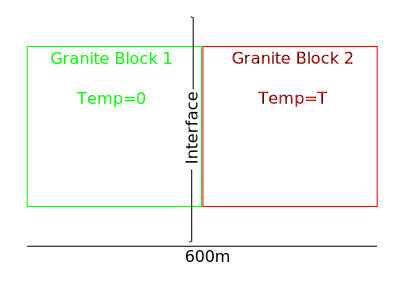
\includegraphics[width=4.in]{figures/onedheatdiff002}}
\caption{Example 2: One dimensional model of an Iron bar}
\label{fig:onedhdmodel}
\end{figure}

This problem is very similar to the example of temperature diffusion in granite
blocks presented in the previous Section~\ref{Sec:1DHDv00}. Thus, it is possible
to modify the script we have already developed for the granite blocks to suit
the iron bar problem.  
The obvious differences between the two problems are the dimensions of the
domain and different materials involved. This will change the time scale of the
model from years to hours. The new settings are
\begin{python}
#Domain related.
mx = 1*m #meters - model length
my = .1*m #meters - model width
ndx = 100 # mesh steps in x direction 
ndy = 1 # mesh steps in y direction - one dimension means one element
#PDE related
rho = 7874. *kg/m**3 #kg/m^{3} density of iron
cp = 449.*J/(kg*K) # J/Kg.K thermal capacity
rhocp = rho*cp 
kappa = 80.*W/m/K   # watts/m.Kthermal conductivity
qH = 0 * J/(sec*m**3) # J/(sec.m^{3}) no heat source
Tref = 20 * Celsius  # base temperature of the rod
T0 = 100 * Celsius # temperature at heating element
tend= 0.5 * day # - time to end simulation
\end{python}
We also need to alter the initial value for the temperature. Now we need to set
the temperature to $T_{0}$ at the left end of the rod where we have
$x_{0}=0$ and 
$T_{ref}$ elsewhere. Instead of \verb|whereNegative| function we now
use \verb|whereZero| which returns the value one for those sample points where
the argument (almost) equals zero and the value zero elsewhere. The initial
temperature is set to
\begin{python}
# ... set initial temperature ....
T= T0*whereZero(x[0])+Tref*(1-whereZero(x[0]))
\end{python}

\subsection{Dirichlet Boundary Conditions}
In the iron rod model we want to keep the initial temperature $T_0$ on
the left side of the domain constant with time. 
This implies that when we solve the PDE~\refEq{eqn:hddisc}, the solution must
have the value $T_0$ on the left hand side of the domain. As mentioned
already in Section~\ref{SEC BOUNDARY COND} where we discussed boundary
conditions, this kind of scenario can be expressed using a
\textbf{Dirichlet boundary condition}. Some people also use the term
\textbf{constraint} for the PDE. 

To define a Dirichlet boundary condition we need to specify where to apply the
condition and determine what value the
solution should have at these locations. In \esc we use $q$ and $r$ to define
the Dirichlet boundary conditions for a PDE. The solution $u$ of the PDE is set
to $r$ for all sample points where $q$ has a positive value.
Mathematically this is expressed in the form;
\begin{equation}
  u(x) = r(x) \mbox{ for any } x \mbox{ with } q(x) > 0
\end{equation} 
In the case of the iron rod we can set
\begin{python}
q=whereZero(x[0])
r=T0
\end{python}
to prescribe the value $T_{0}$ for the temperature at the left end of
the rod where $x_{0}=0$.
Here we use the \verb|whereZero| function again which we have already used to
set the initial value.
Notice that $r$ is set to the constant value $T_{0}$ for all sample
points. In fact, values of $r$ are used only where $q$ is positive. Where $q$
is non-positive, $r$ may have any value as these values are not used by the PDE
solver. 

To set the Dirichlet boundary conditions for the PDE to be solved in each time
step we need to add some statements;
\begin{python}
mypde=LinearPDE(rod)
A=zeros((2,2)))
A[0,0]=kappa
q=whereZero(x[0])
mypde.setValue(A=A, D=rhocp/h, q=q, r=T0)
\end{python}
It is important to remark here that if a Dirichlet boundary condition is
prescribed on the same location as any Neumann boundary condition, the Neumann
boundary condition will be \textbf{overwritten}. This applies to Neumann
boundary conditions that \esc sets by default and those defined by the user.

Besides some cosmetic modification this is all we need to change. The total
energy over time is shown in \reffig{fig:onedheatout1 002}. As heat
is transferred into the rod by the heater the total energy is growing over time
but reaches a plateau when the temperature is constant in the rod, see
\reffig{fig:onedheatout 002}.
You will notice that the time scale of this model is several order of
magnitudes faster than for the granite rock problem due to the different length
scale and material parameters. 
In practice it can take a few model runs before the right time scale has been
chosen\footnote{An estimate of the
time scale for a diffusion problem is given by the formula $\frac{\rho
c_{p} L_{0}^2}{4 \kappa}$, see
\url{http://en.wikipedia.org/wiki/Fick\%27s_laws_of_diffusion}}.

\begin{figure}[ht]
\begin{center}
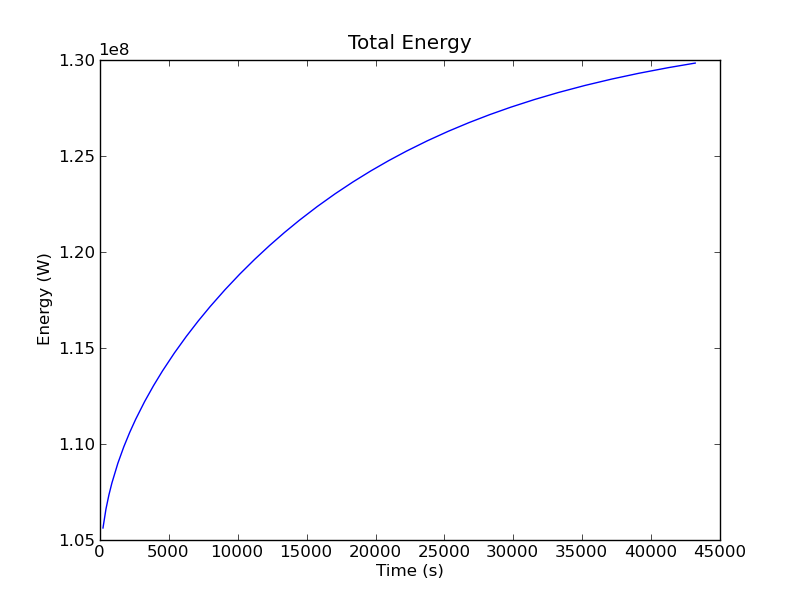
\includegraphics[width=4in]{figures/ttrodpyplot150}
\caption{Example 2: Total Energy in the Iron Rod over Time (in seconds)}
\label{fig:onedheatout1 002} 
\end{center}
\end{figure}

\begin{figure}[ht]
\begin{center}
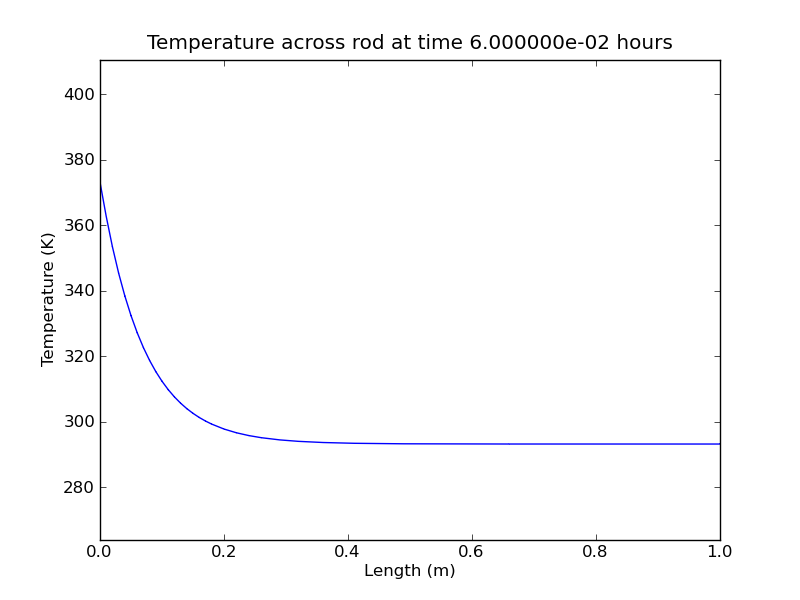
\includegraphics[width=4in]{figures/rodpyplot001}
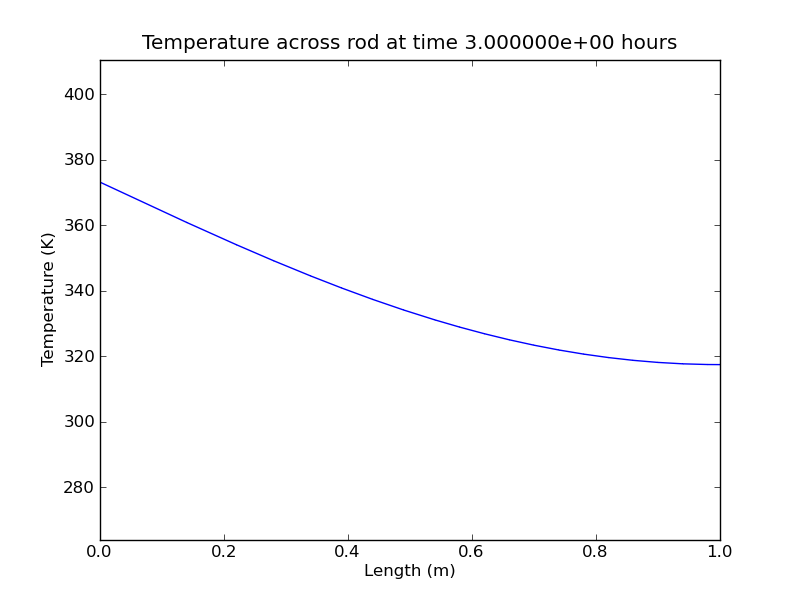
\includegraphics[width=4in]{figures/rodpyplot050}
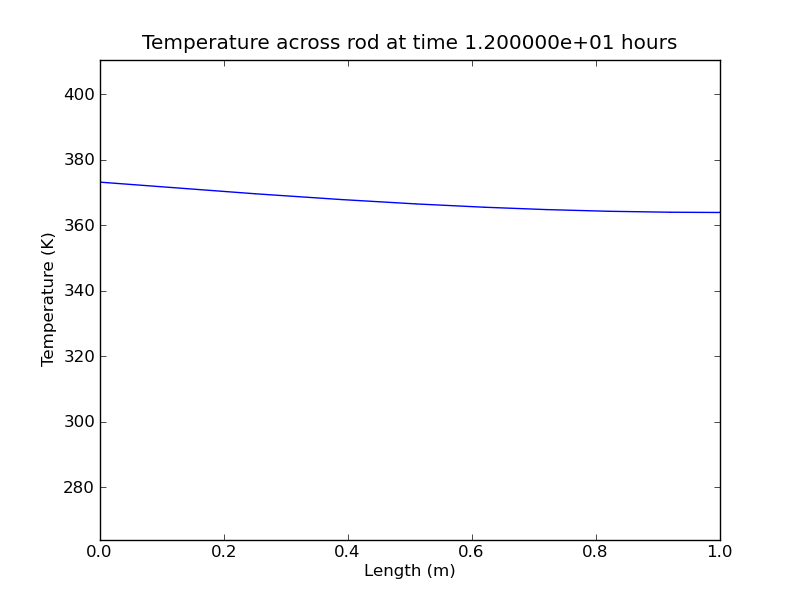
\includegraphics[width=4in]{figures/rodpyplot200}
\caption{Example 2: Temperature ($T$) distribution in the iron rod at time steps
$1$, $50$ and $200$}
\label{fig:onedheatout 002} 
\end{center}
\end{figure}

\section{For the Reader}
\begin{enumerate}
 \item Move the boundary line between the two granite blocks to another part of
the domain.
 \item Split the domain into multiple granite blocks with varying temperatures.
 \item Vary the mesh step size. Do you see a difference in the answers? What
does happen with the compute time?
 \item Insert an internal heat source (Hint: The internal heat source is given
by $q_{H}$.)
 \item Change the boundary condition for the iron rod example such that the
temperature 
 at the right end is kept at a constant level $T_{ref}$, which
corresponds to the installation of a cooling element (Hint: Modify $q$ and
$r$). 
\end{enumerate}

